\newpage % Rozdziały zaczynamy od nowej strony.
\cleardoublepage % Zaczynamy od nieparzystej strony
\pagestyle{headings}
\section{Wstęp}

\subsection{Wprowadzenie}

W ostatnich latach można zaobserwować gwałtowny rozwój w dziedzinie 
Uczenia Maszynowego (ang. \emph{Machine Learning}) i Sztucznej Inteligencji 
(ang. \emph{Artificial Intelligence}). Jednym z algorytmów, który powstał już 
dość dawno, są Sztuczne Sieci Neuronowe (ang. \emph{Artificial Neural 
Networks}). 
Większość algorytmów wykorzystujących Sztuczną Inteligencję wymaga dużej mocy 
obliczeniowej i wyboru odpowiedniego sprzętu. Często powtarzaną operacją matematyczną 
w przypadku algorytmu Sztucznej Sieci Neuronowej jest mnożenie macierzy.
Działanie to można w łatwy sposób zrównoleglić, implementując sieć w układzie 
FPGA i tym samym zwiększyć efektywność algorytmu.

Praca nad implementacją algorytmów Sztucznej Inteligencji w większości 
przypadków zaczyna się od stworzenia i uruchomienia modelu. Do tego zadania 
często wykorzystywane są biblioteki takie jak \emph{Keras} lub \emph{Theano}, które 
w znacznym stopniu przyspieszają proces tworzenia oprogramowania oraz 
ułatwiają wprowadzanie zmian w modelu sieci. Rozwój i dopracowywanie 
algorytmu Sztucznej Inteligencji wymaga wielu iteracji uruchamiania kodu 
z różnymi parametrami i właściwościami sieci.

\subsection{Wstęp teoretyczny}

Temat Sieci Neuronowe ma długą historię rozwoju, sięgającą początku lat 
40. XX wieku, jednak w ostatnich latach można zaobserwować znaczny postęp w tej 
dziedzinie\cite{Kriesel2007NeuralNetworks}. Rozwój technologii umożliwił zastosowanie
algorytmów AI w wielu aplikacjach. 

\subsubsection{Model neuronu}
Sztuczne Sieci Neuronowe to algorytm wzorowany działaniem ludzkiego mózgu 
i znajdujących się w nim neuronów. Model matematyczny pojedynczego 
neuronu — Perceptron \cite{Omondi2006FPGAIO} składa się z wektora wejściowego 
$x = (x_1, x_2,...,x_I)^T$, wektora wag $w = (w_1, w_2,...,w_I)^T$ 
przypisanych do każdego z wejść i funkcji aktywacji $\phi(u)$ 
(Rys. \ref{neuron}). Wyjście neuronu można policzyć według wzoru
$x = (x_1, x_2,...,x_I)^T$, wektora wag $w = (w_1, w_2,...,w_I)^T$.

\begin{figure}[h]
  \centering
  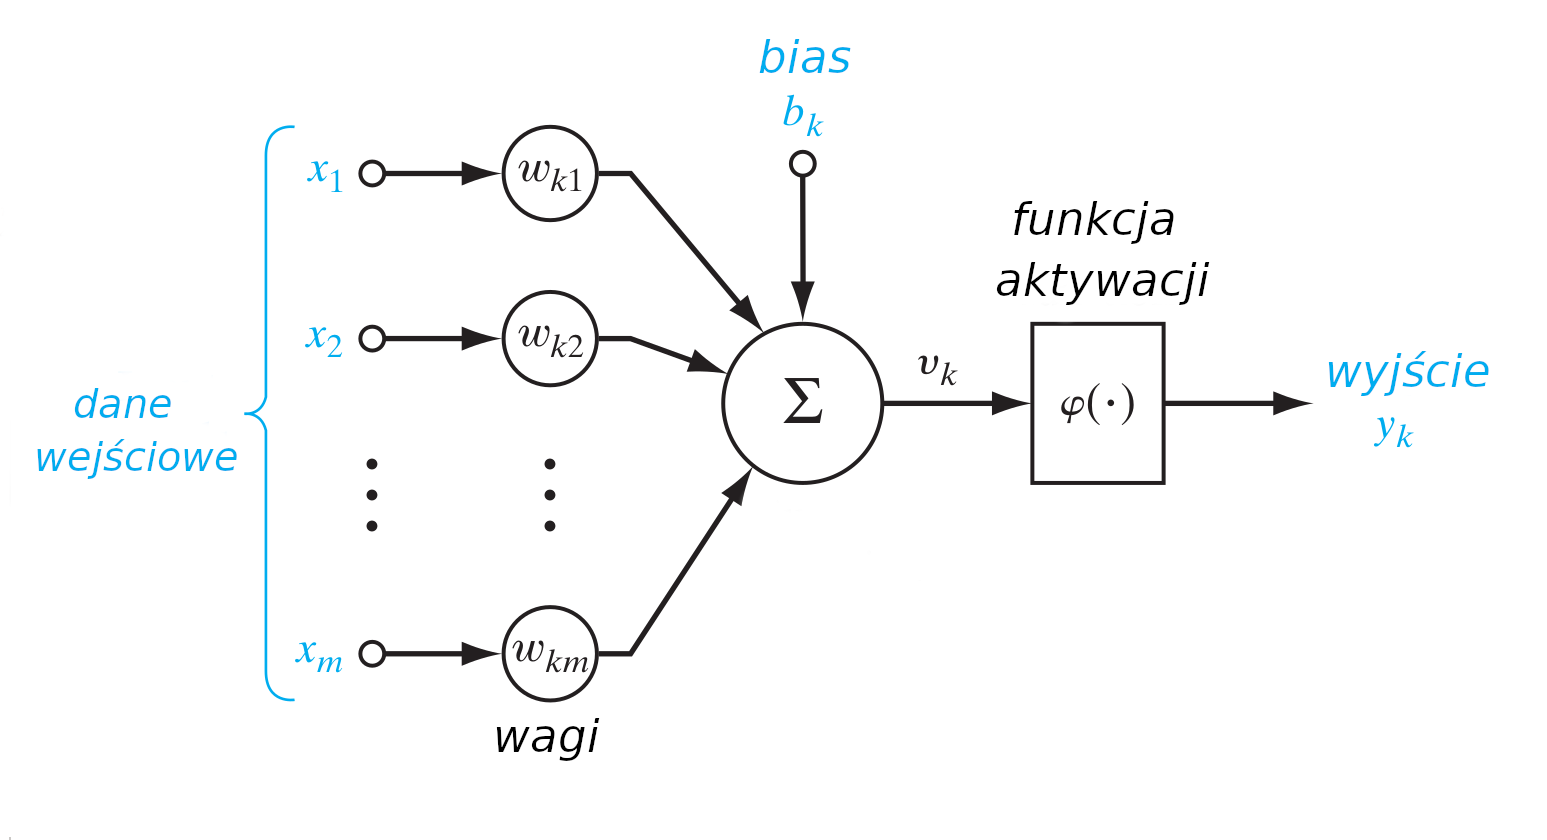
\includegraphics[width=0.8\textwidth]{img/neuron.png}
  \caption{Model pojedynczego perceptronu}
  \label{neuron}
\end{figure}


\subsubsection{Funkcja aktywacji}
Na działanie algorytmu znaczny wpływ może mieć dobór odpowiedniej 
funkcji aktywacji. Wśród najczęściej stosowanych funkcji aktywacji
wyróżnia się:
\begin{itemize}
    \item funkcję ReLu: $\phi(x) = max(0, x)$
    \item funkcję sigmoid: $\phi(x) = \frac{a}{a + e^{-bx}}$
    \item funkcję softmax: $\phi(x_j) = \frac{e^{x_j}}{\sum_{k=1}^{K}{e^{x_k}}}$ dla j = 1,...,N
\end{itemize}

\subsubsection{Perceptron wielowarstwowy}
Jednym z pierwszych modeli Sztucznych Sieci Neuronowych był Perceptron
Wielowarstwowy (ang. MLP — \emph{Multi-Layer Perceptron}), składający 
się z warstwy neuronów wejściowej, ukrytych i wyjściowej (Rys.\ref{mlp}).
Wyjście neuronów w danej warstwie staje się wejściem neuronów warstwy następnej.

Często spotykaną wersją MLP jest model, z warstwami w pełni połączonymi
(ang. FC — \emph{Fully Connected}). W warstwie FC każde z wyjść jest podłączone do 
wszystkich wejść neuronów w warstwie następnej.

\begin{figure}
  \centering
  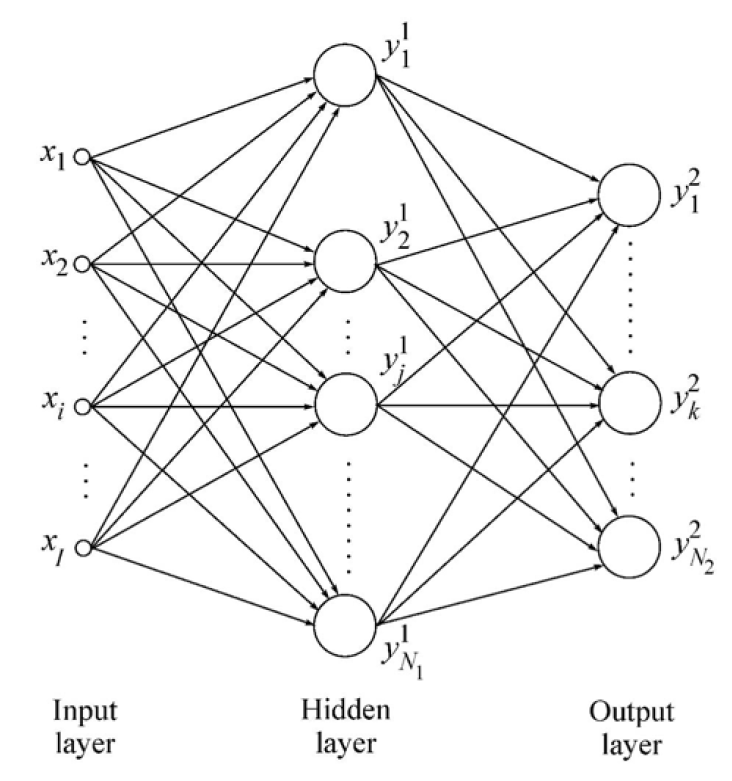
\includegraphics[width=0.5\textwidth]{img/mlp.png}
  \caption{Model Perceptronu Wielowarstwowego}
  \label{mlp}
\end{figure}


\subsubsection{Sieci Głębokie}

Rozwój algorytmów AI doprowadził do powstania Głębokich Sieci Neuronowych (ang. 
\emph{DNN — Deep Neural Networks}), czyli takich, które posiadają wiele 
warstw ukrytych\cite{Goodfellow-et-al-2016}. Algorytm Uczenia Głębokiego (ang. 
\emph{Deep Learning}) umożliwia rozwiązywanie skomplikowanych problemów takich 
jak rozpoznawanie i klasyfikację obiektów na obrazie (Rys.\ref{dnn}). Seria warstw 
ukrytych (ang. \emph{hidden layers}) umożliwia ekstrakcję cech obiektów. 
Kolejne warstwy umożliwiają wykrywanie krawędzi, potem konturów, a na końcu 
całych kształtów i obiektów.

\begin{figure}[!h]
  \centering
  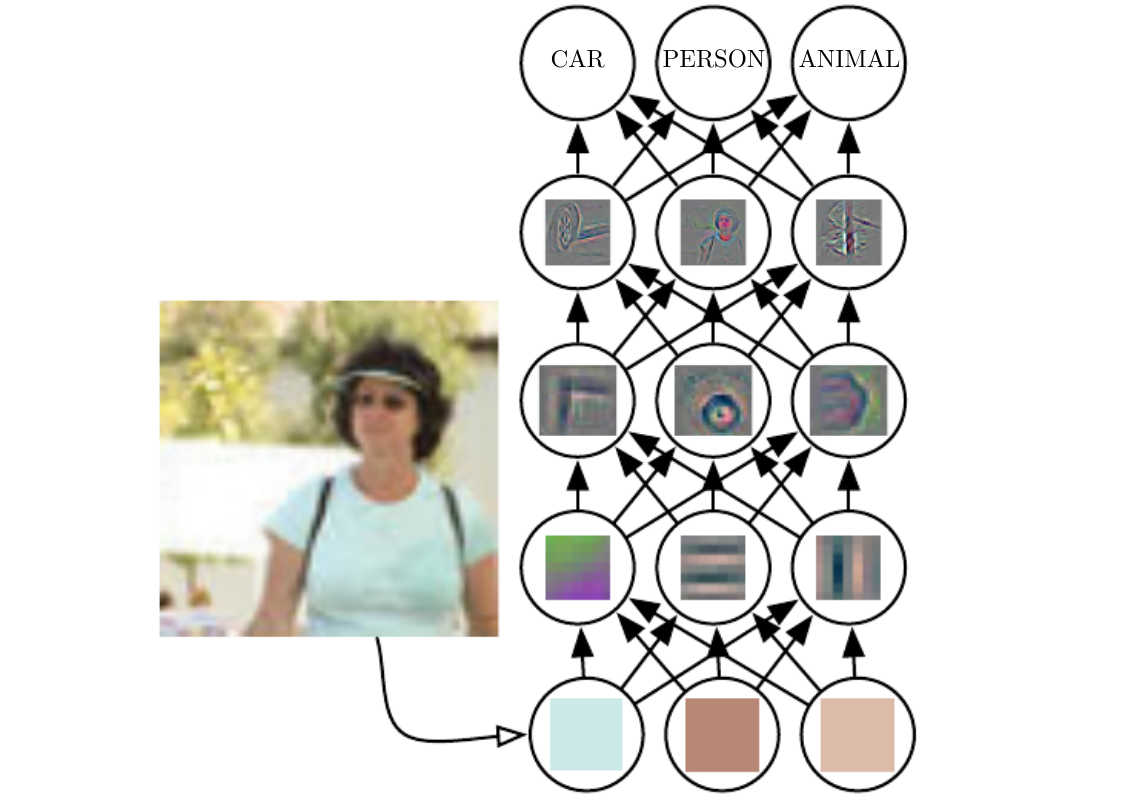
\includegraphics[width=0.8\textwidth]{img/dnn-object-recog.png}
  \caption{Model Głębokiego Uczenia sieci}
  \label{dnn}
\end{figure}


\subsubsection{Wsteczna propagacja błędu}
Architekturę sieci MLP często stosuje się wraz z algorytmem wstecznej 
propagacji błędu (ang. Backpropagation), która umożliwia proces uczenia sieci.
Poprzez obliczenie błędu w neuronach warstwy wyjściowej i propagacji 
wstecz błędu przez całą sieć pozwala dostosować wartość wagi każdej z krawędzi 
w taki sposób, aby zminimalizować wartość funkcji kosztu.

-learning rule (w szczególności delta rule)
-hiperparametry
-uczenie nadzorowane/nienadzorowane
-loss function



\subsection{Implementacja Sztucznych Sieci Neuronowych w układach FPGA}
\subsubsection{Reprezentacja liczb zmiennoprzecinkowych}
\subsubsection{Uczenie Sztucznej Sieci Neuronowej}
\subsection{Zastosowania Sztucznych Sieci Neuronowych}